%%%%%%%%%%%%%%%%%%%%%%%%%%%%%%%%%%%%%%%%%
% Beamer Presentation
% LaTeX Template
% Version 1.0 (10/11/12)
%
% This template has been downloaded from:
% http://www.LaTeXTemplates.com
%
% License:
% CC BY-NC-SA 3.0 (http://creativecommons.org/licenses/by-nc-sa/3.0/)
%
%%%%%%%%%%%%%%%%%%%%%%%%%%%%%%%%%%%%%%%%%

%----------------------------------------------------------------------------------------
%	PACKAGES AND THEMES
%----------------------------------------------------------------------------------------

\documentclass{beamer}

\mode<presentation> {

% The Beamer class comes with a number of default slide themes
% which change the colors and layouts of slides. Below this is a list
% of all the themes, uncomment each in turn to see what they look like.

%\usetheme{default}
%\usetheme{AnnArbor}
%\usetheme{Antibes}
%\usetheme{Bergen}
%\usetheme{Berkeley}
%\usetheme{Berlin}
%\usetheme{Boadilla}
%\usetheme{CambridgeUS}
%\usetheme{Copenhagen}
%\usetheme{Darmstadt}
%\usetheme{Dresden}
%\usetheme{Frankfurt}
%\usetheme{Goettingen}
%\usetheme{Hannover}
%\usetheme{Ilmenau}
%\usetheme{JuanLesPins}
%\usetheme{Luebeck}
\usetheme{Madrid}
%\usetheme{Malmoe}
%\usetheme{Marburg}
%\usetheme{Montpellier}
%\usetheme{PaloAlto}
%\usetheme{Pittsburgh}
%\usetheme{Rochester}
%\usetheme{Singapore}
%\usetheme{Szeged}
%\usetheme{Warsaw}

% As well as themes, the Beamer class has a number of color themes
% for any slide theme. Uncomment each of these in turn to see how it
% changes the colors of your current slide theme.

%\usecolortheme{albatross}
%\usecolortheme{beaver}
%\usecolortheme{beetle}
%\usecolortheme{crane}
%\usecolortheme{dolphin}
%\usecolortheme{dove}
%\usecolortheme{fly}
%\usecolortheme{lily}
%\usecolortheme{orchid}
%\usecolortheme{rose}
%\usecolortheme{seagull}
%\usecolortheme{seahorse}
%\usecolortheme{whale}
%\usecolortheme{wolverine}

%\setbeamertemplate{footline} % To remove the footer line in all slides uncomment this line
%\setbeamertemplate{footline}[page number] % To replace the footer line in all slides with a simple slide count uncomment this line

%\setbeamertemplate{navigation symbols}{} % To remove the navigation symbols from the bottom of all slides uncomment this line
}

\usepackage{graphicx} % Allows including images
\usepackage{booktabs} % Allows the use of \toprule, \midrule and \bottomrule in tables
\usepackage[utf8]{inputenc}
\graphicspath{ {./photos/} }

%----------------------------------------------------------------------------------------
%	TITLE PAGE
%----------------------------------------------------------------------------------------

\title[Seminar]{Identifying Depression with Machine Learning} % The short title appears at the bottom of every slide, the full title is only on the title page

\author{Ivan Lovrenčić} % Your name
\institute[FER] % Your institution as it will appear on the bottom of every slide, may be shorthand to save space
{
University of Zagreb, Faculty of Electrical Engineering and Computing \\ % Your institution for the title page
\medskip
\textit{ivan.lovrencic@fer.hr} % Your email address
}
\date{} % Date, can be changed to a custom date

\begin{document}

\begin{frame}
\titlepage % Print the title page as the first slide
\end{frame}

\begin{frame}
	
	
	\textbf{Identifying Depression on Twitter(2016)}\\
	Authors: M. Nadeem, M. Horn, G. Coppersmith, et al.
	
\end{frame}

\begin{frame}
\frametitle{Overview} % Table of contents slide, comment this block out to remove it
\tableofcontents % Throughout your presentation, if you choose to use \section{} and \subsection{} commands, these will automatically be printed on this slide as an overview of your presentation
\end{frame}

%----------------------------------------------------------------------------------------
%	PRESENTATION SLIDES
%----------------------------------------------------------------------------------------

\section{Motivation}

\begin{frame}
	\frametitle{Motivation}
	
	\begin{itemize}
			\item More people than ever being diagnosed with a mental disorder
			\item Increase of young people with MDD (major depressive disorder)
			\item Mental disorders (specifically, depression) detection has not changed for nearly 50 years
			\item Early depression detection through user's posts on Twitter
	\end{itemize}
	

\end{frame}

\section{Background}

\begin{frame}
\frametitle{Background}

		\begin{itemize}
		\item Rich bodies of work on depression have been performed within the psychiatry, psychology, medicine, and sociolinguistic fields 
		\item \textbf{Shallow ML algorithms + text features}
		\item More recent approaches involve deep learning and topic modeling
		\item Goal: To detect and predict Major Depressive Disorder (MDD) and other mental illnesses
	\end{itemize}



\end{frame}

\section{Machine Learning}

\begin{frame}
	\frametitle{Decision tree}	
	\begin{columns}[c] % The "c" option specifies centered vertical alignment while the "t" option is used for top vertical alignment
		
		\column{.45\textwidth} % Left column and width
		\textbf{Pros}
		\begin{enumerate}
			\item Clarity and interpretable nature
			\item Don't demand a lot of data preparation
			\item Not computationally costly
		\end{enumerate} 
	
		\textbf{Cons}
		\begin{enumerate}
			\item Easy to overfit
			\item Don't perform adequately on more complicated tasks
		\end{enumerate}
		
		\column{.5\textwidth} % Right column and width
		\begin{figure}[h]
			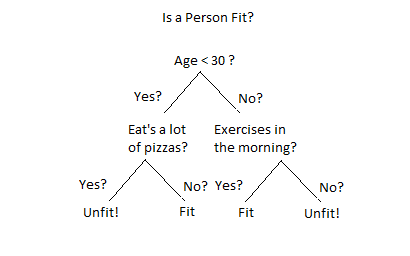
\includegraphics[width=7cm]{decision-tree}
			\caption{An example of simple decision tree}
		\end{figure}
		
	\end{columns}	
\end{frame}

\begin{frame}
	\frametitle{Logistic regression vs Linear regression}	
	
	\begin{columns}[c] % The "c" option specifies centered vertical alignment while the "t" option is used for top vertical alignment
		
		\column{.5\textwidth} % Left column and width
		\textbf{Logistic regression}
		\begin{itemize}
			\item Generalized linear model
			\item Sigmoid function
			\item Probabilistic output
			\item Logistic loss
			\item Iterative optimization
		\end{itemize} 
		
	\column{.5\textwidth} % Left column and width
	\textbf{Linear regression}
	\begin{itemize}
		\item Generalized linear model
		\item Identity function
		\item No probabilistic output
		\item Quadratic loss
		\item Closed-form solution
	\end{itemize} 
	\end{columns}	
\end{frame}

\begin{frame}
	\frametitle{Logistic regression vs Linear regression}	
	\begin{figure}[h]
		\centering
		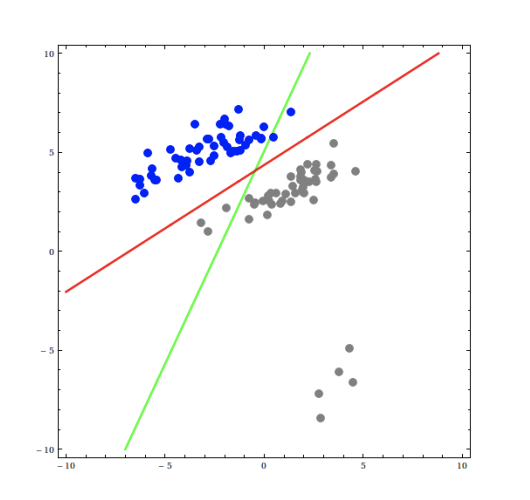
\includegraphics[width=7cm]{logistic}
		\caption{Logistic regression (red line) vs Linear regression (green line)}
	\end{figure}
	
\end{frame}

\begin{frame}
	\frametitle{Logistic regression vs Linear regression}	
	\begin{figure}[h]
		\centering
		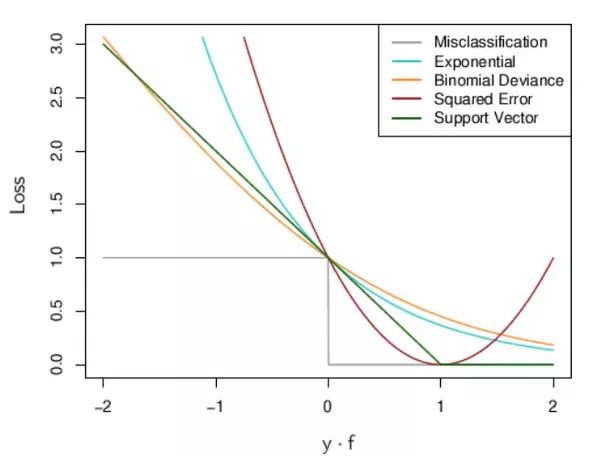
\includegraphics[width=9cm]{losses}
		\caption{Comparison of different loss functions}
	\end{figure}
	
\end{frame}

\begin{frame}
	\frametitle{Support vector machine}	
	\begin{columns}[c] % The "c" option specifies centered vertical alignment while the "t" option is used for top vertical alignment
		
		\column{.5\textwidth} % Left column and width
		\begin{itemize}
			\item Maximum margin hyperplane
			\item Generalization power
			\item Dual vs primary formulation
			\item Hard margin vs soft margin
			\item Hinge loss function
		\end{itemize} 
				
		\column{.45\textwidth} % Right column and width
		\begin{figure}[h]
			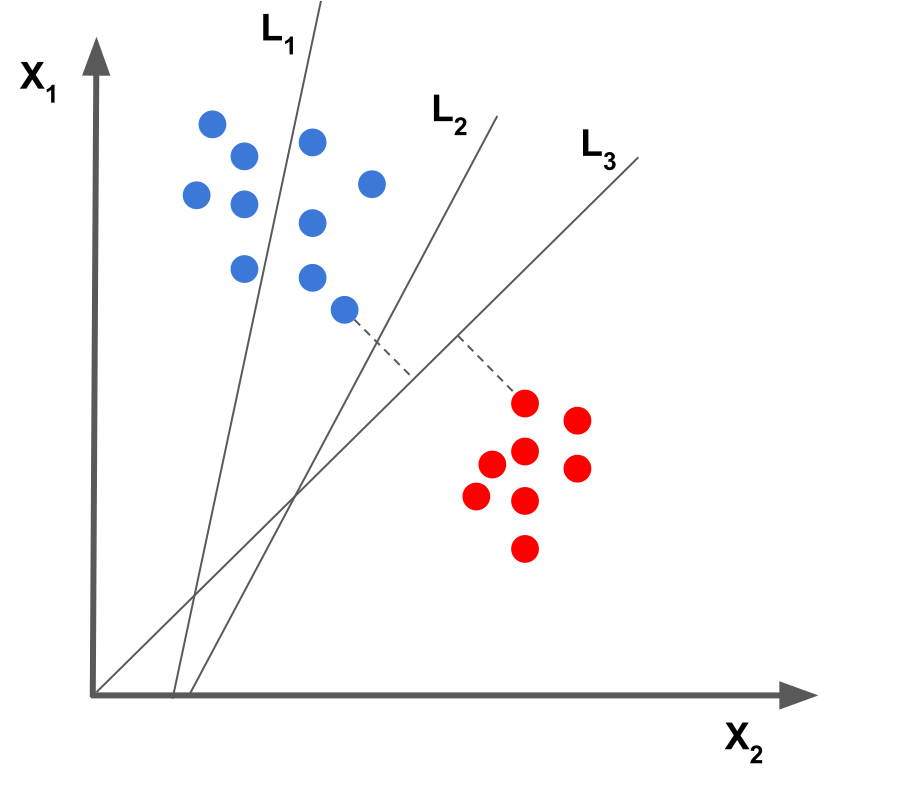
\includegraphics[width=6cm]{svm}
			\caption{L3 model has maximum margin hyperplane}
		\end{figure}
		
	\end{columns}	
\end{frame}

\begin{frame}
	\frametitle{Support vector machine}
	\begin{block}{Dual vs primary formulation}
		$h(x) = w^{T}x + w_0$  = primary formulation 	\newline
		$h(x) = \sum_{i = 1}^{N} \alpha_i y^{i} \textbf{x}^{T}\textbf{x}^{i} + w_0  $  = dual formulation
 	\end{block}
	 
\end{frame}

\begin{frame}
	\frametitle{Support vector machine}	
	\begin{figure}[h]
		\centering
		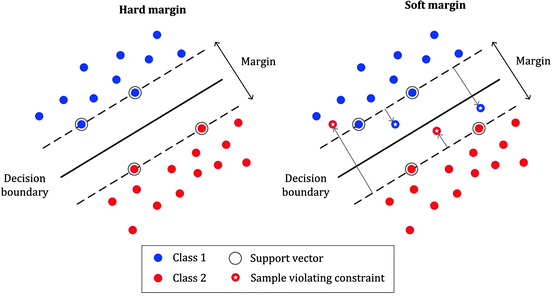
\includegraphics[width=10cm]{margin}
		\caption{Difference between hard-margin (left) and soft-margin (right) model.}
	\end{figure}
	
\end{frame}

\begin{frame}
	\frametitle{Support vector machine}	
	\begin{figure}[h]
		\centering
		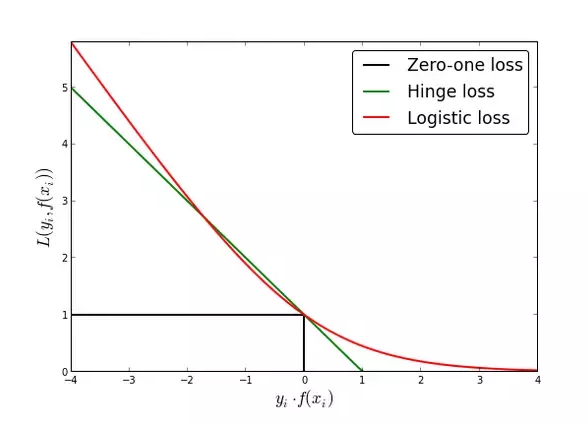
\includegraphics[width=8cm]{hinge-loss}
		\caption{Hinge loss vs logistic loss function}
	\end{figure}
	
\end{frame}

\begin{frame}
	\frametitle{Naive Bayes}	
	\begin{columns}[c] % The "c" option specifies centered vertical alignment while the "t" option is used for top vertical alignment
		
		\column{.5\textwidth} % Left column and width
		\begin{itemize}
			\item Generative probabilistic model
			\item Bayes theorem
			\item Probabilistic output
			\item Parameter estimation - MLE or MAP
		\end{itemize} 
			
		\column{.45\textwidth} % Right column and width
		\begin{figure}[h]
			\centering
			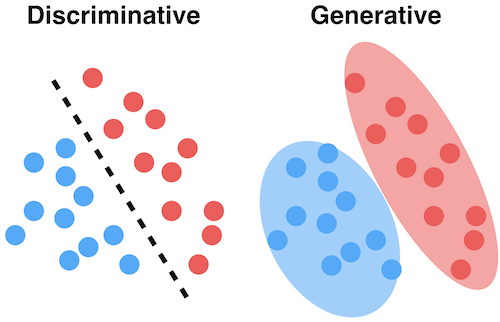
\includegraphics[width=5cm]{discriminative}
			\caption{Discriminative vs Generative model}
		\end{figure}
		
	\end{columns}	
\end{frame}

\begin{frame}
	\frametitle{Naive Bayes}	
	\begin{theorem}[Bayes theorem]
		$P(y|x) = \frac{p(x|y)*P(y)}{P(x)}$ 
	\end{theorem}
	
	\begin{itemize}
		\item $P(y|x)$ - the probability of label $y$ for an example x (a posteriori)
		\item $P(y)$ - the probability of label $y$ (a priori)
		\item $P(x)$ - the probability distribution of the examples
		\item $P(x|y)$ - the probability of example $x$ if there is a label $y$ (likelihood)
	\end{itemize}
\end{frame}

\begin{frame}
	\frametitle{Naive Bayes}	
	\begin{figure}[h]
		\centering
		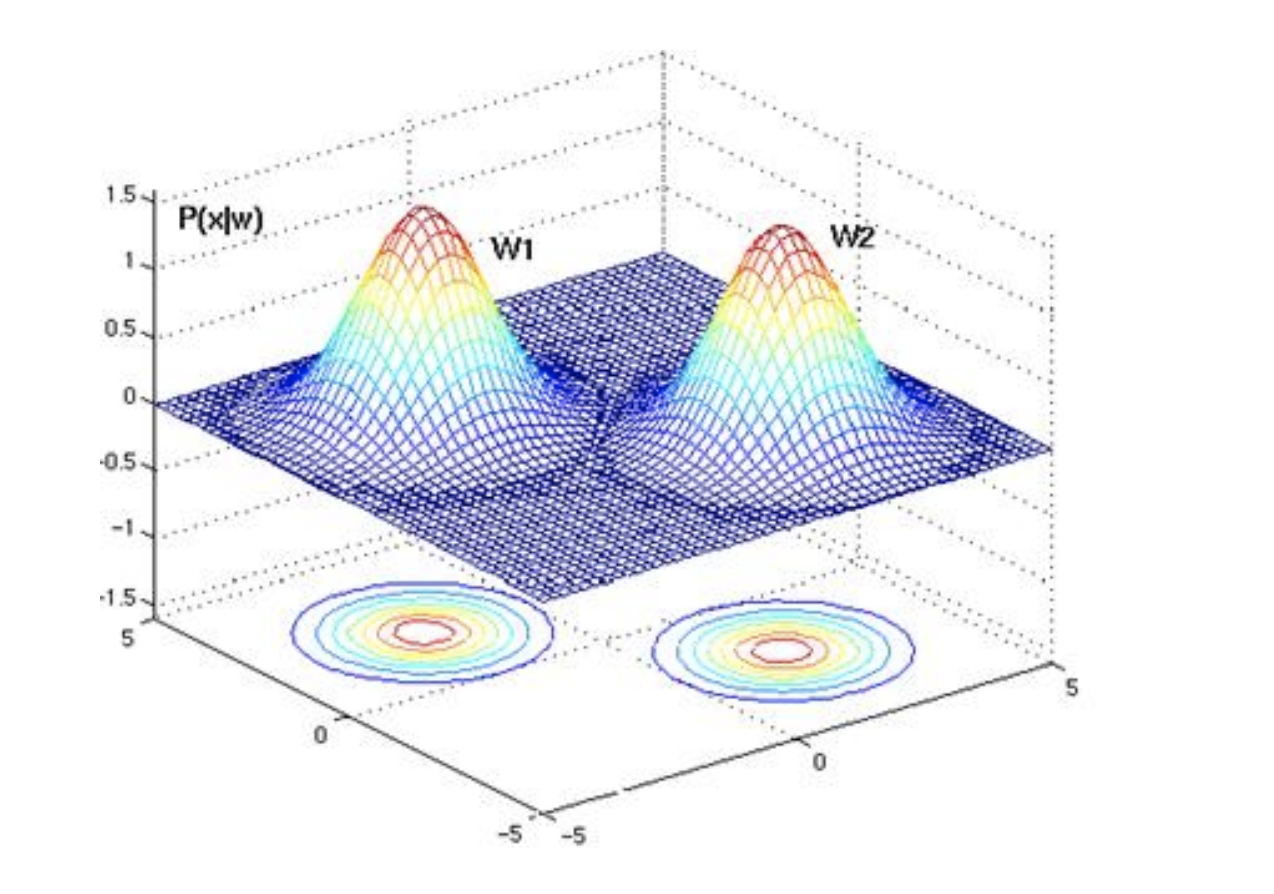
\includegraphics[width=8cm]{bayes}
		\caption{Binary classification with normal distributions for class likelihood}
	\end{figure}
\end{frame}

\section{Dataset  \& Model}

\begin{frame}
	\frametitle{Dataset}	
	
		\begin{table}[h!]
			\centering
			\begin{tabular}{|p{3cm}|p{3cm}|p{3cm}|} 
				\hline
				\multicolumn{3}{|c|}{CLPsych 2015 Twitter dataset}\\
				\hline
				Mental condition & Number of users & Number of tweets \\ [0.5ex] 
				\hline
				No condition & 574 & 1,253,594 \\ 
				Depression & 426 & 742,560 \\
				\hline
				\textbf{Total} & \textbf{1000} & \textbf{2,000,000}\\
				\hline
			\end{tabular}
			\caption{Distribution of the CLPsych 2015 dataset}
			\label{Table:1}
		\end{table}
	
\end{frame}

\begin{frame}
	\frametitle{Dataset}	
	
	\begin{table}[h!]
		\centering
		\begin{tabular}{|p{3cm}|p{3cm}|p{3cm}|} 
			\hline
			\multicolumn{3}{|c|}{Reddit Self-Reported Depression Diagnosis (RSDD) dataset}\\
			\hline
			Data split & Number of users & Number of posts \\ [0.5ex] 
			\hline
			Train & 486 & 295,509 \\ 
			Validation  & 206 & 118,937 \\ 
			Test & 200 & 117,899  \\
			\hline
			\textbf{Total} & \textbf{892} & \textbf{532,345}\\
			\hline
		\end{tabular}
		\caption{Distribution of the RSDD dataset based on data split}
		\label{Table:1}
	\end{table}

\begin{table}[h!]
	\centering
	\begin{tabular}{|p{3cm}|p{3cm}|p{3cm}|} 
		\hline
		\multicolumn{3}{|c|}{Reddit Self-Reported Depression Diagnosis (RSDD) dataset}\\
		\hline
		Mental condition & Number of users & Number of posts \\ [0.5ex] 
		\hline
		No condition & 755 & 450864 \\ 
		Depression  & 137 & 81761 \\ 
		\hline
		\textbf{Total} & \textbf{892} & \textbf{532,345}\\
		\hline
	\end{tabular}
	\caption{Distribution of the RSDD dataset based on mental condition}
	\label{Table:1}
\end{table}
\end{frame}

\begin{frame}
	\frametitle{Dataset}	
	\begin{columns}[c] % The "c" option specifies centered vertical alignment while the "t" option is used for top vertical alignment
		
		\column{.5\textwidth} % Left column and width
		\begin{figure}[h]
			\centering
			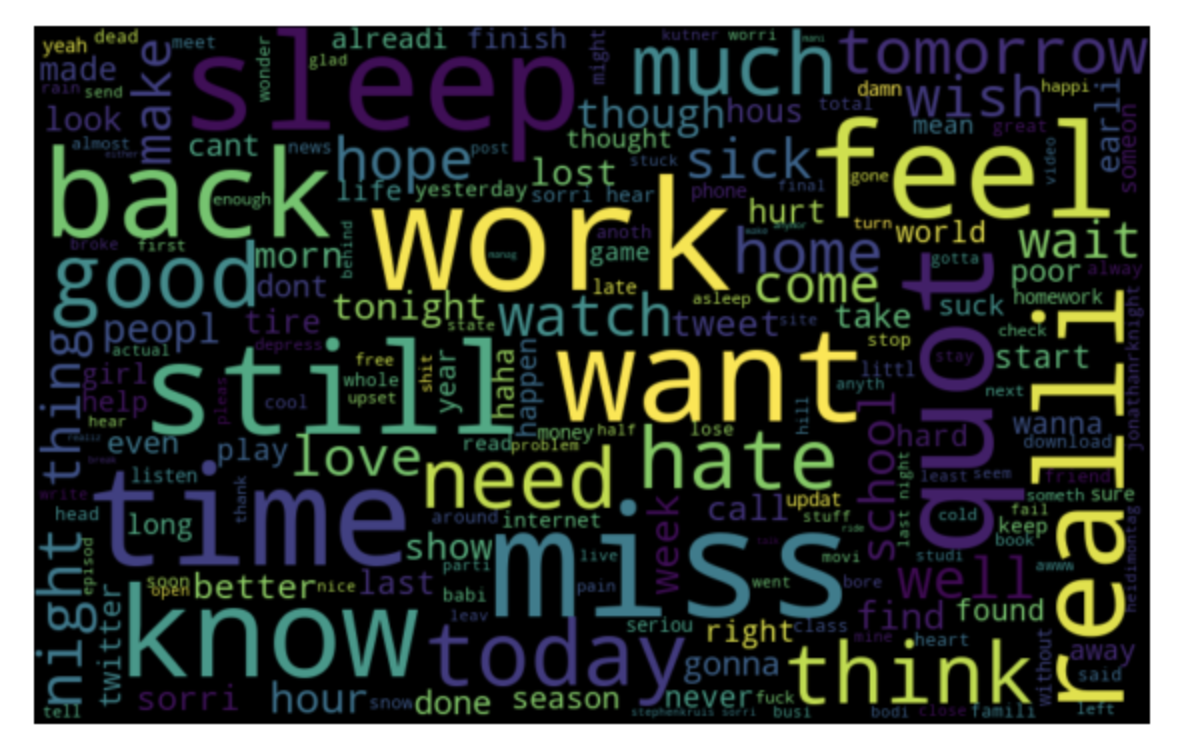
\includegraphics[width=6cm]{words1}
			\caption{Most common words among depressive users in Twitter dataset}
		\end{figure}
		
		\column{.5\textwidth} % Right column and width
		\begin{figure}[h]
			\centering
			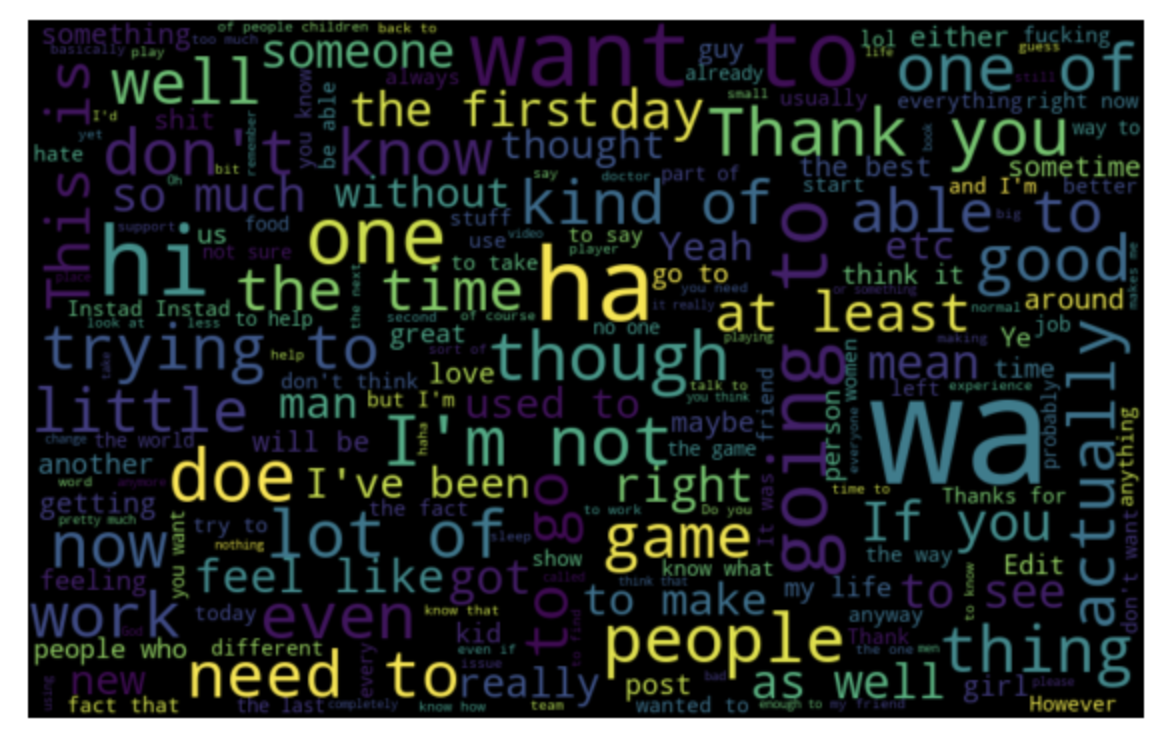
\includegraphics[width=6cm]{words2}
			\caption{Most common words among depressive users in Reddit dataset}
		\end{figure}
		
	\end{columns}	
\end{frame}

\begin{frame}
	\frametitle{Model}	
	\begin{itemize}
		\item Five binary classifiers (shallow ML algorithm + bag-of-words/tf-idf)
		\item Sckit-learn libraries + Python3
		\item RSDD dataset
	\end{itemize}
	
\end{frame}

\section{Results}

\begin{frame}
	\frametitle{Results}	
	\begin{table}[h!]
		\centering
		\begin{tabular}{|p{3cm}|p{1.5cm}|p{1.5cm}|p{1.5cm}|p{1.5cm}|} 
			\hline
			\multicolumn{5}{|c|}{The Johns Hopkins paper results}\\
			\hline
			Algorithm & Precision & Recall & F1-score & Accuracy \\ [0.5ex] 
			\hline
			Decision Trees & 0.67 & 0.68 & 0.75 & 0.67 \\ 
			LinearSVC & 0.83 & \textbf{0.83} & 0.83 & 0.82 \\ 
			Naive Bayes & 0.81 & 0.82 & 0.81 & \textbf{0.86} \\ 
			Logistic &  \textbf{0.86} & 0.82 &  \textbf{0.84} & 0.82 \\ 
			Ridge Classifier & 0.81 & 0.79 & 0.78 & 0.79 \\ 
			\hline
		\end{tabular}
		\caption{The evaluation of the Johns Hopkins models}
		\label{Table:1}
	\end{table}
\end{frame}

\begin{frame}
	\frametitle{Results}	
	\begin{table}[h!]
		\centering
		\begin{tabular}{|p{3cm}|p{1.5cm}|p{1.5cm}|p{1.5cm}|p{1.5cm}|} 
			\hline
			\multicolumn{5}{|c|}{The reimplementation results}\\
			\hline
			Algorithm & Precision & Recall & F1-score & Accuracy \\ [0.5ex] 
			\hline
			Decision Trees & 0.62 & 0.62 & 0.62 & 0.62 \\ 
			LinearSVC & 0.60 & 0.59 & 0.58 & 0.59 \\ 
			Naive Bayes & 0.69 & 0.68 & 0.68 & 0.68 \\ 
			\textbf{Logistic} &  \textbf{0.71} & \textbf{0.70} &  \textbf{0.70} & \textbf{0.70} \\ 
			Ridge Classifier & 0.67 & 0.67 & 0.67 & 0.67 \\ 
			\hline
		\end{tabular}
		\caption{The evaluation of the reimplemented models}
		\label{Table:1}
	\end{table}
	
\end{frame}

%------------------------------------------------

\section{Conclusion}

\begin{frame}
\frametitle{Conclusion}
\begin{itemize}
\item Bag of words + shallow ML performs worse but still adequately on different text format and domain
\item Add more task specific features
\item Explore with deep learning
\end{itemize}
\end{frame}


\begin{frame}
\Huge{\centerline{The End}}
\end{frame}

%----------------------------------------------------------------------------------------

\end{document} 